% !TEX root = ../BeamerTemplate.tex
%%%%%%%%%%%%%%%%%%%%%%%%%%%%%%%%%%%%%%%%%%%%%%%%%%%%%%%%%%%%%%%%%%%%%%%%%%%%%%%%%%

\section{Marco teórico} 
\begin{frame}[fragile]{Divide y vencerás}
    \begin{block}{1. División}Descomponer el problema central en subproblemas independientes más pequeños\end{block}
    \begin{block}{2. Conquista} Resolver cada subproblema de forma recursiva hasta alcanzar  el caso base\end{block}
    \begin{block}{3. Combinación} Fusionar las soluciones de los subproblemas para construir respuesta final\end{block}

\end{frame}


%%%%%%%%%%%%%%%%%%%%%%%%%%%%%%%%%%%%%%%%%%%%%%%%%%%%%%%%%%%%%%%%%%%%%%%%%%%%%%%%%%%%%%

\begin{frame}{Algoritmos implementados}
    \begin{block}{Merge Sort}
        Divide recursivamente el arreglo en dos mitades y luego las fusiona usando arreglos auxiliares. \newline
        
        \textbf{Optimización:} Incorpora un umbral threshold que cambia a Insertion Sort para subarreglos pequeños

    \end{block}

    \begin{block}{Quick Sort}
        Divide el arreglo con partición de Lomuto usando un pivote y ordena recursivamente ambos lados. \newline

        \textbf{Variantes de pivote:} Primero, ultimo, aleatorio y mediana.
    \end{block}

\end{frame}

\begin{frame}{Algoritmos implementados}
    \begin{block}{Búsqueda binaria recursiva}
        Acorta rango de busqueda a la mitad
    \end{block}

    \begin{block}{Búsqueda por interpolación}
        Utiliza la formula $pos = low + \frac{(high - low)}{(arr[high] - arr[low])} * (x - arr[low])$ para estimar la posición del elemento buscado en lugar de dividir el arreglo en mitades.
    \end{block}

    \begin{block}{Búsqueda exponencial}
        Duplica  el límite \texttt{bound *= 2} hasta hallar el rango, luego aplica búsqueda binaria.
    \end{block}

\end{frame}

\begin{frame}{Algoritmos implementados}
    \begin{block}{Búsqueda por rango}
        Usa búsqueda binaria recursiva para encontrar el primer y último índice con el valor objetivo.
    \end{block}

    \begin{block}{Quick Select}
        Encuentra el k-ésimo elemento sin ordenar completamente usando partición recursiva.
        Selecciona pivote mediante mediana de 3 y descarta mitades innecesarias.
    \end{block}

\end{frame}

\begin{frame}[fragile]{Complejidades teóricas}
    \begin{figure}
        \centering
        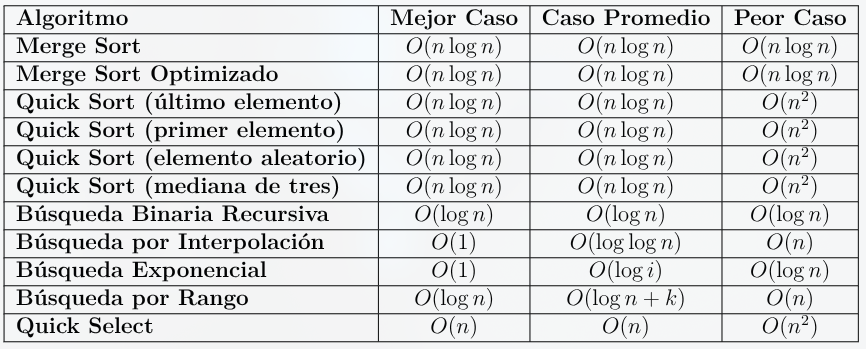
\includegraphics[width=1\textwidth]{AuxiliaryFiles/image.png}
    \end{figure}
\end{frame}

\section{Implementación}

\begin{frame}{Benchmarks}
    $N$ deportistas creciente con $50$ pasos, $5$ repeticiones cada caso (mejor, promedio y peor). Se guardan los promedios en archivos CSV.
    \begin{columns}[T]
        \column{.5\textwidth}
        \begin{block}{Search Benchmark}
            Compara 6 algoritmos de búsqueda en mejor, promedio y peor caso con tamaños crecientes.
        \end{block}

        \begin{block}{Sort Benchmark}
            Evalúa 10 variantes de ordenamiento con intervalos para identificar rendimiento relativo.
        \end{block}

        \column{.5\textwidth}
        \begin{block}{Selection Benchmark}
            Mide Quick Select en mejor y peor caso para encontrar el k-ésimo elemento.
        \end{block}

        \begin{block}{Threshold Benchmark}
            Prueba valores threshold de Merge Sort (2, 4, 8, ..., 128) para optimizar cambio a Insertion Sort.
        \end{block}
    \end{columns}

\end{frame}

\begin{frame}[squeeze]{Otras funcionalidades}
    \begin{columns}[T]
        \column{.5\textwidth}

        \begin{block}{Flujo interactivo}
            Permite elegir algoritmos de ordenamiento y visualizar resultados en tiempo real.
        \end{block}

        \begin{block}{Búsqueda por ID}
            Localiza deportista mediante ID usando diferentes algoritmos de búsqueda.
        \end{block}

        \column{.5\textwidth}
        \begin{block}{Ranking Top N}
            Utiliza \textbf{Quick Select} para encontrar los N mejores deportistas por puntaje.
        \end{block}

        \begin{block}{Rango de puntajes}
            Ordena con \textbf{Quick Sort (mediana)} y aplica \textbf{búsqueda por rango}.
        \end{block}

        \begin{block}{k-ésimo deportista}
            \textbf{Quick Select} para encontrar el k-ésimo deportista sin ordenar.
        \end{block}
    \end{columns}

\end{frame}

\section{Resultados}

\begin{frame}{Sorting secuencial vs divide y vencerás}
    \begin{figure}
        \centering
        
\includegraphics[width=1\textwidth]{AuxiliaryFiles/sort_average_benchmark.pdf}
    \end{figure}
\end{frame}

\begin{frame}{Sorting}
    \begin{columns}[T]
        \column{.5\textwidth}
        \begin{figure}
            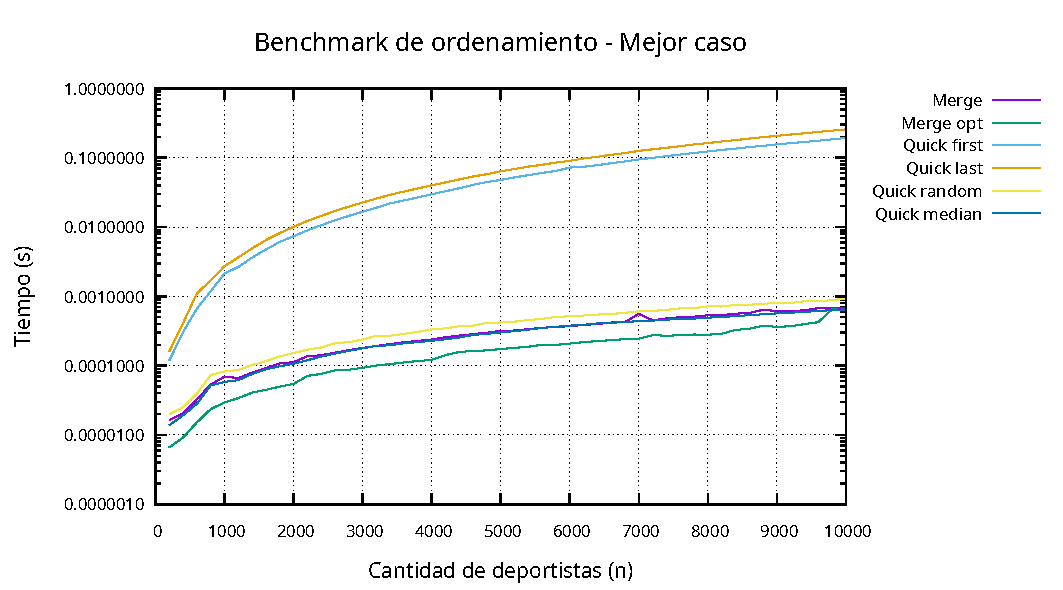
\includegraphics[width=\textwidth]{AuxiliaryFiles/sort_best_benchmark_dyv.pdf}
        \end{figure}

        \column{.5\textwidth}
        \begin{figure}
            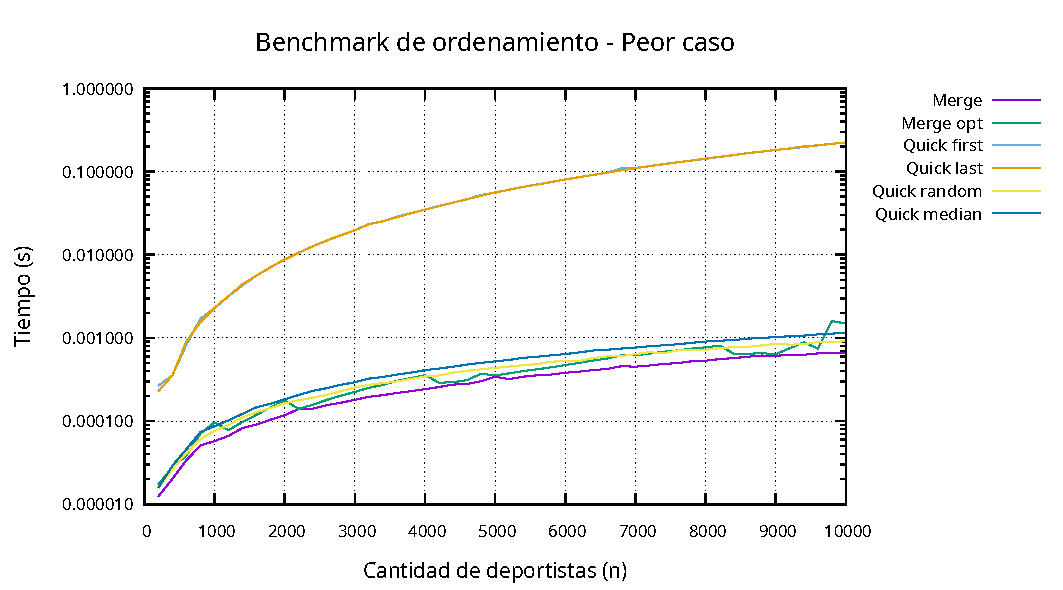
\includegraphics[width=\textwidth]{AuxiliaryFiles/sort_worst_benchmark_dyv.pdf}
        \end{figure}
    \end{columns}

    \begin{figure}
        \centering
        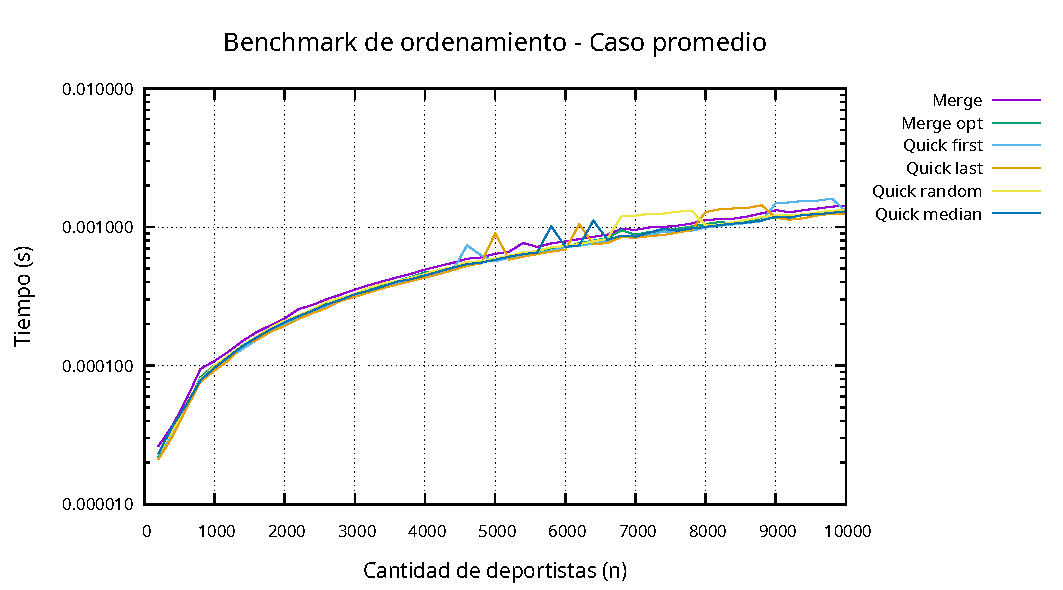
\includegraphics[width=0.5\textwidth]{AuxiliaryFiles/sort_average_benchmark_dyv.pdf}
    \end{figure}

\end{frame}

\begin{frame}{Búsqueda}
    \begin{columns}[T]
        \column{.5\textwidth}
        \begin{figure}
            
\includegraphics[width=\textwidth]{AuxiliaryFiles/search_average_benchmark.pdf}
        \end{figure}

        \column{.5\textwidth}
        \begin{figure}
            
\includegraphics[width=\textwidth]{AuxiliaryFiles/search_worst_benchmark.pdf}
        \end{figure}
    \end{columns}
\end{frame}

\begin{frame}{Quick Select}
    \begin{figure}
        \centering
        
\includegraphics[width=1\textwidth]{AuxiliaryFiles/selection_benchmark.pdf}
    \end{figure}
\end{frame}

\begin{frame}{Threshold de Merge Sort}
    \begin{figure}
        \centering
        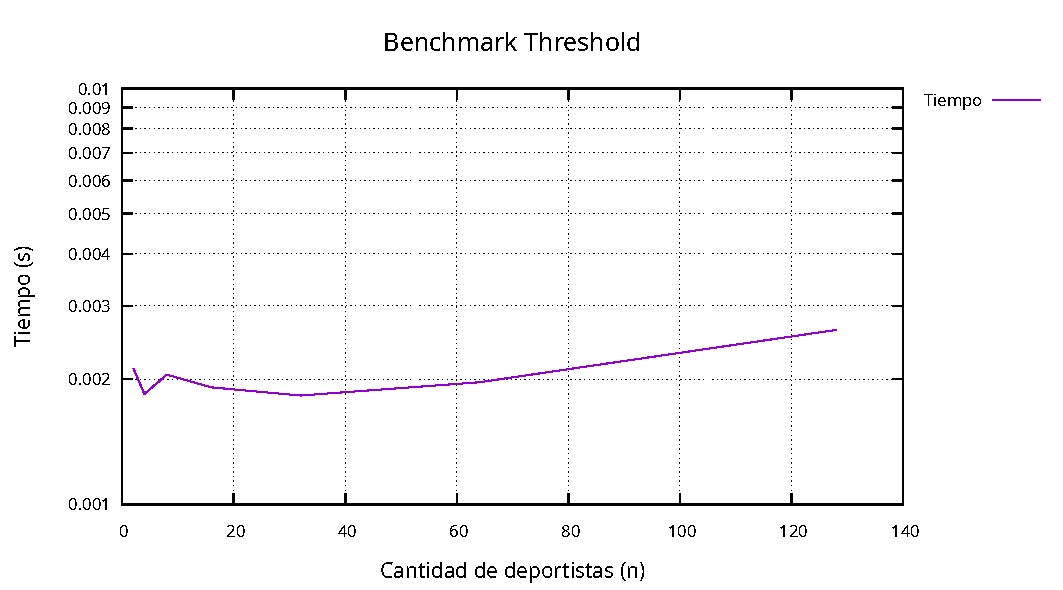
\includegraphics[width=1\textwidth]{AuxiliaryFiles/threshold_benchmark.pdf}
    \end{figure}
\end{frame}

\section{Conclusiones}
\begin{frame}{Conclusiones}
    \begin{itemize}
        \item Merge sort es el algoritmo más eficiente y previsible
        \item En quick sort la elección del pivote es crucial para el rendimiento
        \item La recursión no siempre es la mejor opción para arreglos pequeños como se ve en el benchmark de threshold

    \end{itemize}
\end{frame}